%----------------------------------------------------------------------------------------
%	PACKAGES AND OTHER DOCUMENT CONFIGURATIONS
%----------------------------------------------------------------------------------------

\documentclass[12pt, oneside]{book} % 12 pt font, one-sided book style (each chapter starts on the next page)
%\documentclass[12pt, twoside]{book} % 12 pt font, two-sided book style (each chapter starts on an odd numbered page)

\usepackage[a4paper, includehead, headheight=0.6cm, inner=3cm ,outer=2.5cm, top=2.5 cm, bottom=2.5cm]{geometry}  % Changing size of document
\usepackage[english]{babel} % The document is in English
\usepackage[utf8]{luainputenc} % UTF8 encoding
\usepackage[T1]{fontenc} % Font encoding

%References
\usepackage{csquotes} % required by biber
\usepackage[style=alphabetic, backend=biber, bibencoding=utf8]{biblatex}
\addbibresource{references/report_bibliography.bib}

\usepackage[table,xcdraw]{xcolor} % define colors with label1

\usepackage{graphicx} % For including images
\graphicspath{{./resources/}} % Specifies the directory where pictures are stored

\usepackage{longtable} % tables that can span several pages
\usepackage[bf]{caption} % caption: FIG in bold
\usepackage{fancyhdr} % For the headers

\newcommand{\numberedchapter}{ % Preparation for numbered chapters
	\cleardoublepage % To make sure the previous headers are passed
	\fancyhead[RE]{{\bfseries \leftmark}}% Headers for left pages
	\fancyhead[LO]{{\bfseries \rightmark}}}% Headers for right pages
\newcommand{\unnumberedchapter}[1]{ % Preparation for unnumbered chapters
	\cleardoublepage % To make sure the previous headers are passed
	\addcontentsline{toc}{chapter}{#1} % Also adds the chapter name to the Contents
	\fancyhead[RE]{{\bfseries #1}} % Headers for left pages
	\fancyhead[LO]{}}%Headers for right pages

\usepackage{emptypage} % No headers on an empty page

\usepackage{eso-pic} % For the background picture on the title page
\newcommand\BackgroundPic{%
\put(-180,-160){%
\parbox[b][\paperheight]{\paperwidth}{%
\vfill
\centering

\includegraphics[width=200px]{logos/htw_berlin.jpg}%
\vfill
}}}

\usepackage{hyperref} % Adds clickable links at references

%----------------------------------------------------------------------------------------
%	ADD YOUR CUSTOM VALUES, COMMANDS AND PACKAGES
%----------------------------------------------------------------------------------------

% Open Preamble/mydefinitions.tex and enter some values (name, thesis title...) 
% and include your own custom LaTeX functions and packages

%----------------------------------------------------------------------------------------
%	VALUES FOR THE REPORT
%----------------------------------------------------------------------------------------

\newcommand{\name}{Tim Oelkers} % Author name
\newcommand{\matrikelnr}{s0568352} % Author name
\newcommand{\thesistitle}{AI in der Robotik} % Title of the thesis
\newcommand{\submissiondate}{21. March, 2021} % Submission date "Month, year"
\newcommand{\supervisor}{Patrick Baumann, M.Sc.} % Supervisor name
%\newcommand{\cosupervisor}{} % Co-Supervisor name, comment this line if there is none
\newcommand{\bibliographytitle}{Bibliography}

%----------------------------------------------------------------------------------------
%	YOUR PACKAGES (be careful of package interaction)
%----------------------------------------------------------------------------------------

\usepackage{amsthm,amsmath,amssymb,amsfonts,bbm}% Math symbols
\usepackage[onehalfspacing]{setspace}% 1.5pt line-space
\usepackage[stretch=10]{microtype}%smoother letters
\usepackage{tikz}%vector graphics tikz
\usepackage{wrapfig}% text around figures
\usepackage{subfigure}%graphics including subgraphics
\usepackage{float}%support of H positioning (no automatic placing of elements)
\usepackage{listings}%source code highlighting

%----------------------------------------------------------------------------------------
%	YOUR DEFINITIONS AND COMMANDS
%----------------------------------------------------------------------------------------

% New Commands
\newcommand{\bea}{\begin{eqnarray}} % Shortcut for equation arrays
\newcommand{\eea}{\end{eqnarray}}
\newcommand{\e}[1]{\times 10^{#1}}  % Powers of 10 notation

% Defining a theorem box for Criteria
\newtheorem{critere}{Criterion}
\newcommand{\crit}[2]{
\begin{center}  
\fbox{ \begin{minipage}[c]{0.9 \textwidth}
\begin{critere}
\textbf{\textup{ #1}} --- #2
\end{critere}
\end{minipage}  } \end{center}
}

%\renewcommand*{\labelalphaothers}{} % remove + from references when citating
%\renewcommand{\lstlistlistingname}{Source Code Content} % add chapter 'Source Code Conetent'

% additinal colors for coding adaptions
\definecolor{Ao}{rgb}{0.0, 0.39, 0.0}
\definecolor{antiquefuchsia}{rgb}{0.57, 0.36, 0.51}
\definecolor{bostonuniversityred}{rgb}{0.8, 0.0, 0.0}
% coding adaptions for better visibility (can be overwritten)
\renewcommand{\lstlistingname}{Code snippet}
\lstset{
	language=python,
	numbers=left,
	columns=fullflexible,
	aboveskip=5pt,
	belowskip=10pt,
	basicstyle=\small\ttfamily,
	backgroundcolor=\color{black!5},
	commentstyle=\color{black},
	morecomment=[s]{.s}{hape}, % workaround to exclude ".shape"
	keywordstyle=\color{antiquefuchsia},
	otherkeywords={self, else},
	emphstyle=\color{bostonuniversityred},
	emph={shape,units,name,filters,kernel_size,activation,padding,kernel_initializer,kernel_regularizer,bias_initializer,inputs,outputs,mode,distribution,minval,maxval, callback_args, low, high, limit, window_length, size, mu, theta, sigma},
	stringstyle=\color{Ao},
	showspaces=false,
	showstringspaces=false,
	showtabs=false,
	xleftmargin=16pt,
	xrightmargin=0pt,
	framesep=5pt,
	framerule=1pt,
	frame=leftline,
	rulecolor=\color{black},
	tabsize=2,
	breaklines=true,
	breakatwhitespace=true
}


\begin{document}

%----------------------------------------------------------------------------------------
%	TITLE PAGE
%----------------------------------------------------------------------------------------

\pagestyle{empty} % No page numbers
\frontmatter % Use roman page numbering style (i, ii, iii, iv...) for the preamble pages

\begin{titlepage}
\AddToShipoutPicture*{\BackgroundPic}
\begin{center}
\vfill
{\large \scshape University of Applied Sciences Berlin\textsl{}}\\[1.4cm]
{\Large Report}\\[0.5cm]
\rule{\textwidth}{1.5pt}\\[0cm]
{\huge \bfseries \thesistitle \par \ }\\[-0.5cm]
\rule{\textwidth}{1.5pt}\\[2.5cm]
\hfill  by\\[1cm]
\hfill  {\large \bfseries\name}\\
\hfill  {\large \bfseries\matrikelnr}\\
\vfill
{\hfill \large Supervisor: \textbf{\supervisor}} \\ 
\ifx\cosupervisor\undefined\else{\hfill \large Co-Supervisor: \textbf{\cosupervisor}} \\ \fi
\vspace{1cm}
\hfill  \submissiondate
\end{center}
\end{titlepage}

%----------------------------------------------------------------------------------------
%	PREAMBLE PAGES (comment out unnecessary pages)
%----------------------------------------------------------------------------------------

\pagestyle{fancy} % Changes the headers
\renewcommand{\chaptermark}[1]{ \markboth{#1}{}} % Getting the chapter name right
\renewcommand{\sectionmark}[1]{\markright{\thesection\; #1}} % Getting the section name right
\fancyhf{}% Clears header and footer
\fancyhead[RO,LE]{\thepage} % page number on the outside of headers

\unnumberedchapter{Abstract} 
\chapter*{Abstract} 
\subsection*{\thesistitle}

This should be a single paragraph of not more than 500 words, which concisely summarizes the entire proposal.


%----------------------------------------------------------------------------------------
%	LIST OF CONTENTS/FIGURES/TABLES
%----------------------------------------------------------------------------------------

\unnumberedchapter{Contents}
\tableofcontents % Write out the Table of Contents

%----------------------------------------------------------------------------------------
%	THESIS MAIN TEXT - CHAPTERS
%----------------------------------------------------------------------------------------

\addtocontents{toc}{\vspace{2em}} % Add a gap in the Contents, for aesthetics
\mainmatter % Begin numeric (1,2,3...) page numbering

% Import your chapters here
\numberedchapter
\chapter{Introduction}
examples citations:
\\
scientific \cite{doi:10.1162/neco.1989.1.4.541}
\\
general online \cite{LSVRC}
\\
git \cite{chollet2015}
\\

\section{Motivation}
TODO

\section{Project Objective}
TODO

\section{Proceeding and Structure of the Work}
TODO
\chapter{Fundamentals}

\section{Robot Operating System}
ROS (Robot Operating System) is an open-source meta operating system. It runs on top of Unix based systems and 
provides abstraction over process management, low-level communication and hardware. It also provides tools and 
libraries to develop applications in the field of robotics and distributed systems. ROS is build on the concept 
of creating a (possibly distributed) peer-to-peer network of nodes. A node is a single, modular process that 
should perform a dedicated task, which is implemented using C++ (roscpp) or Python (rospy). All nodes register 
themselfs at the ROS master, which serves as a nameserver and processer manager to the rest of the network. 
Nodes communicate which each other using ROS messages, which are data structures that define 
the type of data that is passed. The communication is usually based on ROS topics, 
which implement an asynchronous publish-subscribe pattern so that nodes are truly decoupled. 
If direct, synchronous communication with an immediate response is needed, ROS services can be used.

\section{Neural Networks}
Neural networks are a emulation of a human brain with inter-connected nodes (neurons) with weighted edges (synapses). 
The learning part comes from the process of altering each weight after each evaluation to better map inputs to their 
expected outputs. This is called supervised learning and inputs with known outputs have to be available for that.
During the forward pass, the data passes through the network while the weights are applied. To achieve non-linear mappings, 
an activation function is applied to inputs between each layer. After that, the error to the expected value is 
calculated with a predefined loss function and the weights are updated accoring to a predefined optimizer in a process 
called back-propagation. The process is repeated for a certain number of epochs so that the output gets closer and closer 
to the expected value. After the training, the model can be used on unknown input.

\subsection{Fully Connected Neural Network}
A fully connected network is a type of network where each node of one layer is connected to each node on the following layer.
It is often divided into a input layer, multiple hidden layer and one output layer, which has to have the same number
of nodes as the amount of classes in the classification.

\subsection{Convolutional Neural Networks}
Convolulation neural networks are often used in classification problems and are a specialisation of full connected neural networks. They are escpecially used 
in image and audio classification. It tries to find features or patterns in the provided data by removing noise and extracting data relevant for the actual target. 
They are constructed with a convolutional layer and a pooling layer. The convolutional parts moves a kernel filter over the input matrix and calculates the inner product of
surrounding datapoints. This creates an overlap and helps neighboring neurons react to similiar data (e.g. similiar frequencies in audio data). In the pooling layer, 
the amount of data gets reduced, for example by using max-pooling, a process where only the most active neuron in a certain area is kept and the rest being discarded.
This prevents the model from overfitting (valueing data not actualy relevant for the classification task) and improves training times. The data, now reduced to
its features, is then passed through a fully connected layer for the actual classification.

\chapter{Conception}

\section{Dataset}
For this projects, the "SpeechCommands"\cite{warden2018speech} dataset will be used. This dataset was created by Pete Warden, 
working for Google, with the intent of creating a fundamental set of simple commands spoken in English with a lot of variance. 
The data was gather publicly and thus contains audio from different speakers with normal day-to-day audio quality and possibly even background noise. 
Even though the data comes from a public source, its correctness was checked manually and with various alghorhithms to remove too quiet or interrupted words. 
In total, the data contains 105.829 audio files (3.4 GB) for 35 words spoken by 2.618 different people. All audio files are exacly one seconds long and the data is alligned 
so that words all start and end roughly at the same time. The audio comes in the WAVE format with 16bit single channel (mono) values, sampled at a rate of 16kHz.
The dataset also contains audio files containing common background noise, that can be used for evaluation. The dataset is split into multiple subsets for 
training, testing and validation, specified by specific file lists in the same folder.

\section{Model} \label{model}
The model will be a deep convolutional neural network with 5 convolutional layers described as M5 \cite{dai2016deep}. This was choses as they claim a reasonable high accurary of
over 60% in a 10 class audio classification with a training time of a minute per epoch. They use a very high sampling rate of 32kHz and a very aggresive reduction of the temporal
resolution in the first layer with a kernel size (or receptive field) of 80, a stride of 4 and a ouput size of 128. After each layer, a batch normalization
and a maxpooling of size 4 is performed, further reducing the feature maps. After the first layer, the kernel size is reduced to a more normal size of 3 and the stride reduced to 1.
The heavy reduction of resolution is complemented by a doubling of the amount of filters each layer. They use ReLU as the activation function. While most classification
problems use multiple connected layers after the convolutional layers, the authors claim to use a "fully convolutional design" without fully connected layers. Instead, they
use a global average pooling to reduce the feature maps to a single dimension. At the end, a softmax function is applied.

\section{Audio Capture} \label{audio_capture}
As the quality should be evaluated with a real microphone, the \texttt{audio_capture} ROS package is used for this project. It can be started as a ROS node
and exposes the two topics \texttt{/audio} and \texttt{/audio_info}. The first contains the raw audio data as unsigned 8 bit arrays, the second contains metadata about
how the data should be interpreted. Concretly, it contains the number of channels, the sample rate, the bitrate, the sample format and the encoding format.
How the data correlates to the sampled data is controlled via the encoding format (e.g. 16LE means that two bytes in the little endian format make up one sample).
The data for each channel is stored in an interleaved format and contains no header information. The sample rate specifies how often the analog audio signal from
the microphone is converted to a digital signal. The higher it is, the better the quality (e.g. CD audio is sampled at 44kHz). Of couse, the bit rate, 
mainly specified in kilo bits per second (kbps), has to be high enough to allow for that amount of information to be processed, otherwise the higher sample rate is nullified. 
For uncompressed audio, the bit rate can be calculated by multiplying sample rate, byte count per sample and number of channels.

\section{Evaluation Architecture}
The evaluation architecture will be developed as a ROS application as it helps with development and models a potential real world use case as close as possible. 
The following image shows a graph of the architecture and how the nodes interact with each other.

\begin{figure}
  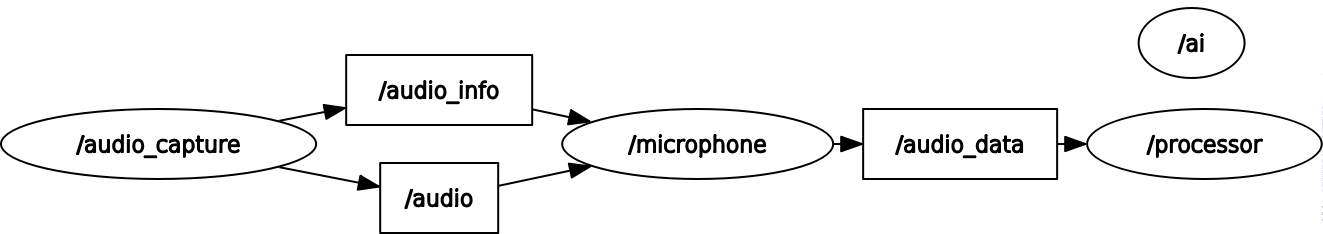
\includegraphics[width=\linewidth]{rosgraph.png}
  \caption{ROS architecture}
  \label{fig:rosgraph}
\end{figure}

As described in section \ref{audio_capture}, the raw audio data and metadata get sent to two topics that are subscribed by the microphone node. It is responsible 
for recording the data when a specific user input has been made. Once another input was made, the data has to be aggregated and sent to the \texttt{audio_data} topic. It is 
subscribed by the processor node, which handles the necessary conversions so that it is compatible with the input of the model. It then also invokes the ai service
which predicts the command and sends it back, together with the probability. To do that, the ai node has to load the pretrained model and metadata about the
used model like the labels it can predict and the used sample rate. The predicted command will then be shown on the console for now.

\chapter{Implementation}

\section{Model Training}
The implementation for the model training is based on a tutorial on command recognition by the pytorch team\cite{tutorial}. The first step is to create a training and 
testing subsets of the whole dataset, that got downloaded and saved locally if needed. The testing and validation filenames are stored in specific files, everything not
listed in these files is supposed to be for training. The iteration and downloading of these files is done by the SPEECHCOMMANDS class provided by torchaudio. The dataset class
also has some methods to get the labels, the amount of files and the sample rate of the subset. As these methods require iteration over all files and thus take some time to compute, 
the results were memoized by implementing a file based cache with the help of pythons object serialization (pickle). This speeds up consecutive model trainings. One datapoint
then contains the waveform, the sample rate, the label, a speaker id and the label number. As I am only able to do the training on the CPU, the audio gets resampled
to 8kHz to improve training time. We then use a standard torch DataLoader and specify a batch count, the number of workers and that the data should be shuffled after each
epoch so that the order is not affecting the model in any way. A so called collate function is also defined that pads the waveforms with zeroes so that all have the same length, encodes
the label as the index in the label array and throws away the rest of the unnwanted data in the dataset (like the sample rate). The model is implemented according to section \ref{model} with
a input size equal to the number of labels. We use the Adam optimizer with a relatively high learning rate of 0.01 and a small weight decay of 0.0001 as in the original paper \cite{dai2016deep}.
The loss function used is called NLLLoss, which is often used in 1D classification problems. The model is then trained and tested for 6 epochs. After that, the model itself 
and metadata about it (labels and sample rate) are saved to disk, together with a graph showing the accuracy and the loss for each epoch.

\section{Evaluation Environment}
All nodes are started via the following launch file. It describes where the nodes are located and how they should be configured. For the audio\_capture node, we have to
match the setup from the original dataset as closely as possible. Thats why we use the WAVE audio format, as it stores the data uncompressed. We also use mono audio
and store the data in the 16 bit little endian format. Even though the audio will be resampled to 8kHz to fit the models sample rate, the initial sample rate should
be as high as possible as during resampling, the average is calculated and we don´t want the higher variation during lower sample rates. The default bitrate set by
the audio\_capture package has to be overwritten to match the expected amount of data.

\lstset{language=XML}
\begin{lstlisting}
<launch>
  <node name="ai" pkg="ros_ai_report" type="ai.py" output="screen"/>
  <node name="microphone" pkg="ros_ai_report" type="microphone.py" output="screen"/>
  <node name="processor" pkg="ros_ai_report" type="processor.py" output="screen"/>
  <node name="audio_capture" pkg="audio_capture" type="audio_capture" output="screen">
    <param name="bitrate" value="256"/>
    <param name="channels" value="1"/>
    <param name="sample_rate" value="16000"/>
    <param name="format" value="wave"/>
    <param name="sink" value="appsink"/>
    <param name="sample_format" value="S16LE"/>
  </node>
</launch>
\end{lstlisting}

The microphone node then stores the received data in memory when a specific key is pressed and joins it together when pressed again. It also calculates the
sample width by extracting the information from the sample format. The processor node receives the aggregated data and writes it to file using the wave module
of the python standard library. This is sadly needed, as torchaudio does not support loading of file-like objects and only expects a string as a file path. The 
needed metadata like sample rate and sample width are received from the microphone node. The ai node loads the model and its metadata from disk. When a request
comes in, it loads the file previously created, resamples the audio to the models sample rate and predicts the command using the model. As the model applies a softmax
function at the end, the data represents the logarithm of the probability of being a certain command. That means, that the highest number is the predicted output
and by applying the exponential function, the probability is calculated. As the highest element is just the index of the command, the actual command has to
be found in the label array stored in the models metadata. The entire process is repeated until the user terminates the program.

\chapter{Evaluation}

First of all, the accuracy of the model was tested agaist the testing subset provided by the used dataset. The following groups of images show the loss (left) and
the accuracy (right) at each epoch.

\begin{figure}[H]
\centering
\begin{minipage}{.45\textwidth}
  \centering
  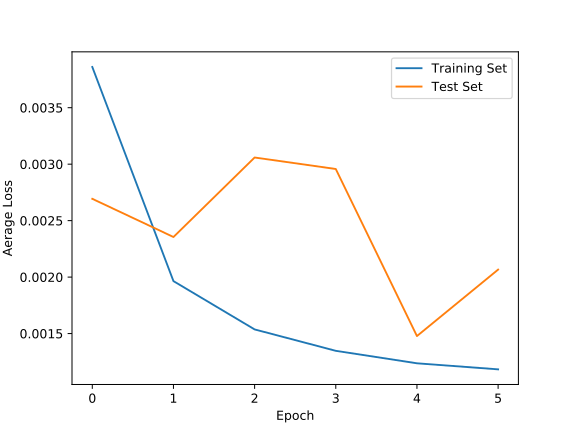
\includegraphics[width=\linewidth]{model_losses_default.png}
  \caption{Default Model Losses}
\end{minipage}
\begin{minipage}{.45\textwidth}
  \centering
  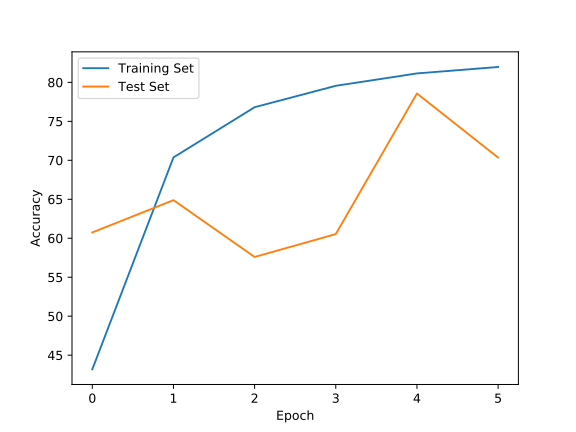
\includegraphics[width=\linewidth]{model_accuracies_default.png}
  \caption{Default Model Accuracies}
\end{minipage}
\end{figure}

Interestingly, the testing accuracy seems to fluctuate and even decreases by a bit at the end while the training accuracy still keeps growing. But still, with
the testing dataset reaching a 78.1\% accuracy and the training dataset reaching a accuracy of 82.5\%, the goal is definetly reached. For reference, the same model
is tested against the validation dataset to see if there are differences in data quality.

\begin{figure}[H]
\centering
\begin{minipage}{.45\textwidth}
  \centering
  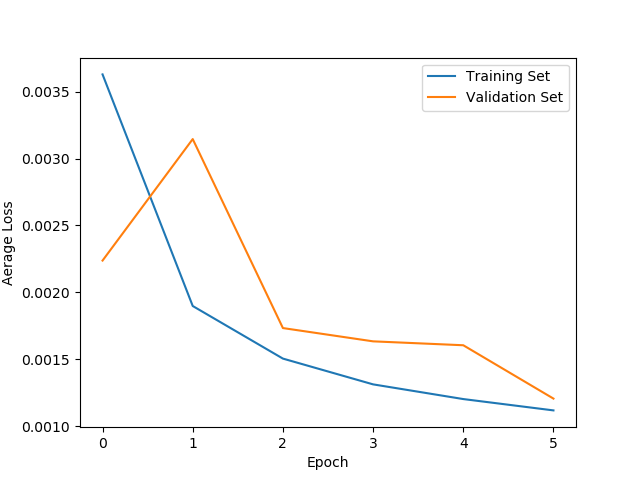
\includegraphics[width=\linewidth]{model_losses_validation.png}
  \caption{Default Model Losses}
\end{minipage}
\begin{minipage}{.45\textwidth}
  \centering
  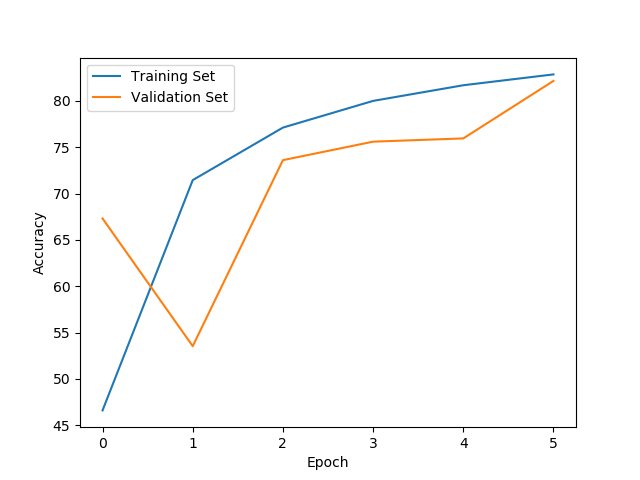
\includegraphics[width=\linewidth]{model_accuracies_validation.png}
  \caption{Default Model Accuracies}
\end{minipage}
\end{figure}

Here, a bit smoother curve for the validation dataset can be seens with the training set reaching 82.9\% and the validation set reaching 82.2\%. With the relativly small epoch
count and it being relativly close to the testing accuracy, it is concluded that no difference in data quality exists.
\chapter{Conclusion}
* length is really important for training, original data is aligned and even padded with zeroes so that all have the same length,
that is not the case for the data coming from the microphone, 
* the model took the waveform at specifc times into consideration, not fully based on the overall structure of the wave

\section{Summary}
TODO

\section{Future Work}
TODO

% clear page and begin capital roman numbering
\clearpage
\pagenumbering{Roman}

%----------------------------------------------------------------------------------------
%	FIGURES, TABLES & CODINGS
%----------------------------------------------------------------------------------------

% List of Figures
\listoffigures
\addcontentsline{toc}{chapter}{List of Figures}
\newpage
% List of Tables
\listoftables
\addcontentsline{toc}{chapter}{List of Tables}
\newpage
% Source Code Content
\lstlistoflistings 
\addcontentsline{toc}{chapter}{Source Code Content}
\newpage

%----------------------------------------------------------------------------------------
%	BIBLIOGRAPHY
%----------------------------------------------------------------------------------------

% filters are not necessary here but kept due copy-paste
\defbibfilter{scientific}{
	type=article or
	type=inbook or
	type=book or
	type=unpublished or
	type=inproceedings or
	type=incollection or
	type=manual or
	type=phdthesis
}

\printbibliography[heading=bibintoc, filter=scientific, title={\bibliographytitle}]\clearpage
\printbibliography[heading=bibintoc, keyword={online}, title={Online References}]\clearpage
\printbibliography[heading=bibintoc, keyword={image}, title={Image References}]\clearpage

%----------------------------------------------------------------------------------------
%	APPENDICES
%----------------------------------------------------------------------------------------

\addtocontents{toc}{\vspace{2em}} % Add a gap in the Contents, for aesthetics
\appendix % Starts of appendices

\numberedchapter
\chapter{About Appendices} \label{appA}


Appendices are optional and should only be used if necessary.

%\input{MainText/appendixB}
%\input{MainText/appendixC}

\end{document}  